\documentclass[11pt,a4paper]{article}
\usepackage{tikz}
\usetikzlibrary{arrows.meta,positioning}
\usepackage{tabularx}
\usepackage{amsmath,amssymb,amsthm}
\usepackage{geometry}
\geometry{margin=1in}
\usepackage{hyperref}
\usepackage{graphicx}
\usepackage{setspace}
\onehalfspacing

\title{\textbf{Paper A-08: Earth Pollution:\\ A Constraint-Driven Flux Dynamics (CDFD) Perspective}}
\author{Steve Bico Mujjabi, MD\\
\small Independent Researcher\\
\small Founder, Vura Labs\\
\small Kampala, Uganda\\
\small ORCID: 0009-0001-0556-5516}
\date{August 2026}

\begin{document}
\maketitle

% BEGIN SHARED-METHODS POINTER
\noindent\textit{Shared Part IV notation and evidence boundaries are defined in \path{PART_IV_METHODS_AND_CLAIM_BOUNDARY.md}. This paper states only its local observables, comparison, and failure conditions.}
% END SHARED-METHODS POINTER


\begin{abstract}
This paper develops a falsifiable CDFD/AFL model of Earth Pollution. It maps chemical, particulate, thermal, biological, and noise loads to driving flux $\Phi$, dilution, adsorption, transformation, and clearance capacity to active constraint $C$, bioremediation, sequestration, treatment, and pathway rerouting to responsiveness $S$, and bioaccumulation, sediment reservoirs, tissue burden, and legacy waste to structural memory $M_s$. The target outcome is exposure, toxicity, transport distance, and recovery, tested against emissions inventories, water and air monitoring, biomarkers, sediments, and ecotoxicology. The paper treats universality as a shared model architecture rather than an assertion that unlike systems have the same material mechanism. It states the negative result that would make the mapping unnecessary and places the domain claim inside the cumulative CDFD programme and its reproducible runtime boundary.
\end{abstract}

\section{Introduction}

A healthy ecosystem is a fluid network operating in thermodynamic equilibrium. Natural waste products, such as fallen leaves or animal remains, represent chemical flux that is immediately processed and recycled by detritivores and microbial networks.

When humans introduce synthetic pollutants (e.g., microplastics, heavy metals, or persistent organic pollutants), they are injecting a massive, highly structured flux into an ecosystem that possesses absolutely no topological pathways to process it. In CDFD terms, pollution (maladaptive $C$ accumulation) is an informational and energetic throughput that faces an infinite natural constraint.

\section{The Bioremediation Adaptive Surface}
We govern the environmental processing capacity using the Adaptive Operating Ratio:
\begin{equation}
    \Psi_s = \left( \frac{\Phi}{C} \right) \cdot S \cdot M_s
\end{equation}

For a contaminated ecological zone (e.g., a river basin or a soil horizon):
\begin{itemize}
    \item \textbf{Flux ($\Phi$)}: The incoming rate of synthetic toxins and heavy metals.
    \item \textbf{Constraint ($C$)}: The chemical resistance to degradation. Synthetic polymers possess extremely high chemical bonds that natural enzymes cannot easily break, acting as a massive biological friction limit.
    \item \textbf{Responsiveness ($S$)}: The bioremediation capacity of the local microbial and fungal communities attempting to adapt and evolve to consume the novel flux.
    \item \textbf{Memory ($M_s$)}: Bioaccumulation and environmental persistence. Because the toxins cannot be processed, they physically accumulate in the tissue of apex predators and the soil matrix. This permanently locks the system into a degraded, toxic state.
\end{itemize}

\subsection{Bioaccumulation as Topological Ischemia}
When natural organic flux enters the system, $C$ is low, and $S$ processes it efficiently ($\Psi_s \approx 1$).

When a synthetic pollutant enters, the local constraint $C$ is effectively infinite. The biological network cannot degrade it. Consequently, the pollutant remains in the system. The physical presence of the toxin actively destroys the underlying microbiota and apex species, dropping the systemic responsiveness $S$ toward zero.

Because the toxin persists, the systemic memory $M_s$ becomes locked into a state of chronic poisoning. The entire network enters a severe bottleneck ($\Psi_s \ll 1$). The ecosystem ceases to function as an active thermodynamic conduit and instead becomes a stagnant, necrotic sink for industrial waste.



\section{Measurement Layer}

% BEGIN PART IV MAJOR CROSS-DOMAIN UPGRADE
\section{Cross-Domain Model Upgrade: Mechanism, Scale, and Tests}

\subsection{Observable Translation}

The paper-specific translation begins with an observable chain rather than a
verbal analogy. For Earth Pollution, the proposed drive is chemical, particulate, thermal, biological, and noise loads.
The active limitation is dilution, adsorption, transformation, and clearance capacity. Responsiveness is carried by
bioremediation, sequestration, treatment, and pathway rerouting, while retained state is represented by
bioaccumulation, sediment reservoirs, tissue burden, and legacy waste. The outcome to explain is exposure, toxicity, transport distance, and recovery.

\begin{table}[htbp]
\centering
\small
\caption{Operational CDFD/AFL map for Paper A-08.}
\begin{tabularx}{\textwidth}{|l|X|X|}
\hline
\textbf{Term} & \textbf{Paper-specific observable meaning} & \textbf{Measurement question} \\
\hline
$\Phi$ & chemical, particulate, thermal, biological, and noise loads & What rate, load, gradient, or demand enters the focal system? \\
\hline
$C$ & dilution, adsorption, transformation, and clearance capacity & Which measured bottleneck limits transfer, function, or recovery? \\
\hline
$S$ & bioremediation, sequestration, treatment, and pathway rerouting & Which process changes effective capacity or reroutes the load? \\
\hline
$M_s$ & bioaccumulation, sediment reservoirs, tissue burden, and legacy waste & Which retained state makes equal present loads produce different futures? \\
\hline
$Y$ & exposure, toxicity, transport distance, and recovery & Which outcome is predicted out of sample, with uncertainty? \\
\hline
\end{tabularx}
\end{table}

\begin{figure}[htbp]
\centering
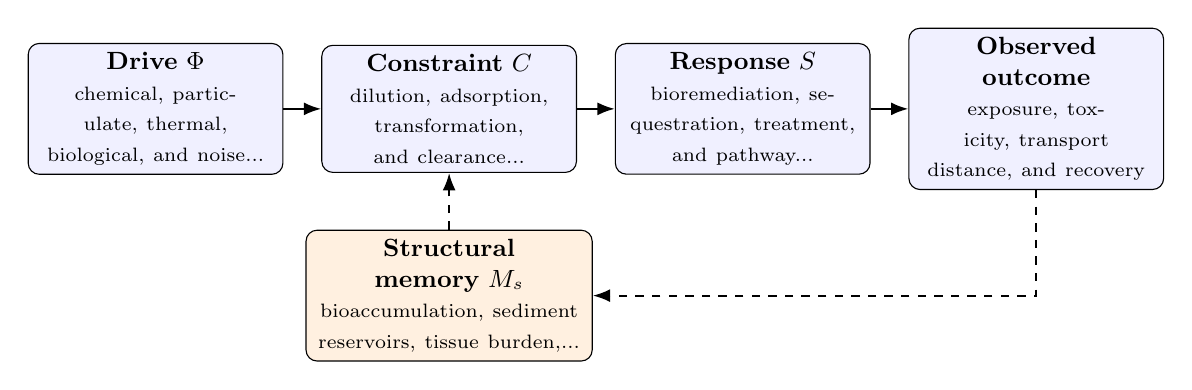
\begin{tikzpicture}[
    node distance=0.48cm,
    every node/.style={font=\small},
    box/.style={draw, rounded corners, align=center, minimum height=1.45cm, text width=3.0cm, fill=blue!6},
    memory/.style={draw, rounded corners, align=center, minimum height=1.25cm, text width=3.4cm, fill=orange!12},
    flow/.style={-{Latex[length=2.2mm]}, thick},
    feedback/.style={-{Latex[length=2.2mm]}, thick, dashed}
]
\node[box] (drive) {\textbf{Drive $\Phi$}\\\scriptsize chemical, particulate, thermal, biological, and noise...};
\node[box, right=of drive] (constraint) {\textbf{Constraint $C$}\\\scriptsize dilution, adsorption, transformation, and clearance...};
\node[box, right=of constraint] (response) {\textbf{Response $S$}\\\scriptsize bioremediation, sequestration, treatment, and pathway...};
\node[box, right=of response] (outcome) {\textbf{Observed outcome}\\\scriptsize exposure, toxicity, transport distance, and recovery};
\node[memory, below=0.72cm of constraint] (memory) {\textbf{Structural memory $M_s$}\\\scriptsize bioaccumulation, sediment reservoirs, tissue burden,...};
\draw[flow] (drive) -- (constraint);
\draw[flow] (constraint) -- (response);
\draw[flow] (response) -- (outcome);
\draw[feedback] (outcome.south) |- (memory.east);
\draw[feedback] (memory.north) -- (constraint.south);
\end{tikzpicture}
\caption{Paper A-08 observable CDFD/AFL architecture for Earth Pollution. Solid arrows give the proposed forward chain; dashed arrows make history-dependent feedback explicit.}
\label{fig:a08-architecture}
\end{figure}

\subsection{Paper-Specific Causal Hypothesis}

For this paper, the hypothesized causal sequence is specific. A change in
chemical, particulate, thermal, biological, and noise loads arrives faster than bioremediation, sequestration, treatment, and pathway rerouting can compensate.
This raises or redistributes dilution, adsorption, transformation, and clearance capacity. If the load persists,
the retained state encoded by bioaccumulation, sediment reservoirs, tissue burden, and legacy waste changes the next response, so a later event of equal
magnitude can produce a different trajectory in exposure, toxicity, transport distance, and recovery. The
scientific task is to estimate that sequence against the best ordinary model of
the domain, not merely to redescribe the outcome after it occurs.

\subsection{Cross-Scale Translation Without Mechanistic Erasure}

For the Earth systems family, the cross-domain translation compares coupled transport, finite environmental capacity, buffering, and retained landscape or ecosystem state. It cannot erase conservation laws, geometry, or scale; it must expose where those domain equations create comparable overload and recovery structures. \cite{Holling1973,Turing1952,BakTangWiesenfeld1987}
The required scale declaration for this paper is minutes to centuries; organisms to airsheds and watersheds. At short
scales, the key question is whether the incoming drive is transmitted,
buffered, or diverted. At intermediate scales, response changes effective
capacity and network exposure. At long scales, retained structure can alter the
state space itself. A result is genuinely cross-scale only when the aggregation
rule is stated and the same conclusion is not an artifact of averaging.

\subsection{Evidence Ladder and Discriminating Tests}

\begin{table}[htbp]
\centering
\small
\caption{Evidence ladder for Paper A-08. Each rung can fail independently.}
\begin{tabularx}{\textwidth}{|p{0.17\textwidth}|X|X|}
\hline
\textbf{Test} & \textbf{Design} & \textbf{Discriminating result} \\
\hline
Proxy audit & Measure emissions inventories, water and air monitoring, biomarkers, sediments, and ecotoxicology and preregister how each record maps to $\Phi$, $C$, $S$, $M_s$, and $Y$. & The mapping fails if proxies are non-identifiable, circular, or change meaning across cases. \\
\hline
Load ramp & Apply or observe a controlled contaminant pulse and subsequent source removal while estimating the dominant constraint and response time. & A threshold claim requires a reproducible nonlinear change and uncertainty bounds, not a visually chosen breakpoint. \\
\hline
Recovery and memory & Match present load across units with different histories, then compare recovery paths. & The memory claim requires history-dependent divergence after current conditions are controlled. \\
\hline
Model comparison & Compare the baseline domain model with and without the CDFD/AFL state variables using held-out data. & The paper's stated falsifier is: legacy and responsiveness terms fail to improve exposure or recovery forecasts. \\
\hline
\end{tabularx}
\end{table}

\subsection{Research Programme and Boundary Conditions}

The immediate research programme has four steps. First, construct a documented
dataset from emissions inventories, water and air monitoring, biomarkers, sediments, and ecotoxicology and retain raw units before normalization.
Second, fit a baseline domain model and report its calibration and out-of-sample
error. Third, add the smallest identifiable CDFD/AFL state extension and test
whether it improves prediction of exposure, toxicity, transport distance, and recovery. Fourth, repeat the
analysis across the declared scale range and publish negative cases as part of
the cross-domain translation audit.

% END PART IV MAJOR CROSS-DOMAIN UPGRADE

\section{Conclusion}
pollution (maladaptive $C$ accumulation) is the thermodynamic equivalent of a biological stroke. It is the injection of an anomalous flux into a network that lacks the topological architecture to process it. By framing environmental toxicity within the CDFD ontology, we frame the hypothesis that ecological collapse from pollution (maladaptive $C$ accumulation) is the model-predicted failure mode of overwhelming the biosphere's structural constraint limitations.
\section*{Conflict of Interest} The author declares no conflict of interest.
\section*{Data Availability}
Part-specific runtime diagnostics are under each Part's \path{outputs/} directory.

Release-wide code: \path{Part_E_Synthesis/supplementary/}.

Generated summaries: \path{Part_E_Synthesis/outputs/}.

Figures: \path{Part_E_Synthesis/figures/}.


\section{Reference Layer}
\bibliographystyle{plain}
\bibliography{universal_afl_references}
\end{document}
